
\begin{figure}[t]
	\centering
	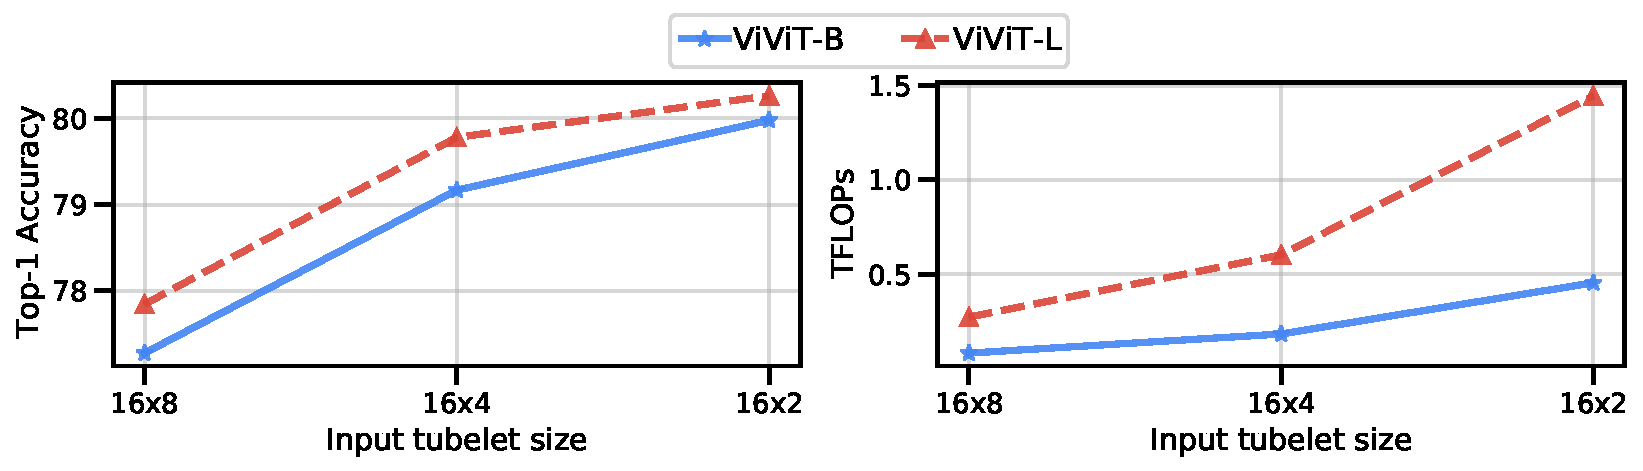
\includegraphics[width=\linewidth]{figures/ablation/patch_size_backbone}
	\footnotesize{
    	\begin{tabularx}{\linewidth}{YY}
    	    (a) Accuracy   &  (b) Compute
    	\end{tabularx}
	}
	\caption{The effect of the backbone architecture on (a) accuracy and (b) computation %
	on Kinetics 400, for the spatio-temporal attention model (Model 1).
	}
	\label{fig:ablation_backbone}
	\vspace{-0.5\baselineskip}
\end{figure}